\documentclass[12pt, a4paper]{book}

\usepackage[T1]{fontenc}
\usepackage[utf8]{inputenc}
\usepackage[charter, cal=cmcal]{mathdesign}
\usepackage[scaled=0.92]{helvet}
\usepackage{geometry}
\geometry{a4paper, top=30mm, bottom=30mm, inner=32mm, outer=25mm, marginparwidth=18mm}

\usepackage{amsmath, amsthm}
\usepackage[version=4]{mhchem}
\usepackage{graphicx}
\usepackage[dvipsnames,svgnames,table]{xcolor}
\usepackage{tikz}
\usetikzlibrary{arrows.meta, shapes.geometric, positioning,
                calc, backgrounds, patterns}
\usepackage{pgfplots}
\pgfplotsset{compat=1.18}
\usepackage{tcolorbox}
\tcbuselibrary{skins, breakable, theorems}
\usepackage{titlesec}
\usepackage{fancyhdr}
\usepackage{enumitem}
\usepackage{booktabs}
\usepackage{array}
\usepackage{multicol}
\usepackage{caption}
\usepackage{parskip}
\usepackage{siunitx}
\usepackage{pifont}
\usepackage{colortbl}
\usepackage[colorlinks=true, linkcolor=BrickRed,
            urlcolor=NavyBlue, citecolor=ForestGreen]{hyperref}

% ── Colours (Journey 3 — forest green / teal) ─────────────────────────────────
\definecolor{JourneyColor}{HTML}{145A32}
\definecolor{ModuleColor}{HTML}{1E8449}
\definecolor{PuzzleColor}{HTML}{1A5276}
\definecolor{DiscoveryColor}{HTML}{B7950B}
\definecolor{WarningColor}{HTML}{C0392B}
\definecolor{ProblemColor}{HTML}{4A235A}
\definecolor{ReflectColor}{HTML}{117A65}
\definecolor{HistoryColor}{HTML}{6E2F1A}
\definecolor{LightBg}{HTML}{F8F9FA}
\definecolor{TableMetal}{HTML}{AED6F1}
\definecolor{TableNonmetal}{HTML}{A9DFBF}
\definecolor{TableNoble}{HTML}{D2B4DE}
\definecolor{TableMetalloid}{HTML}{FAD7A0}
\definecolor{PredictedCell}{HTML}{FADBD8}
\definecolor{GapCell}{HTML}{FDFEFE}

% ── Boxes ─────────────────────────────────────────────────────────────────────
\newtcolorbox{puzzlebox}[1][]{enhanced,breakable,
  colback=PuzzleColor!6,colframe=PuzzleColor,fonttitle=\bfseries\sffamily,
  title={The Puzzle},attach boxed title to top left={yshift=-2mm,xshift=6mm},
  boxed title style={colback=PuzzleColor},borderline west={3pt}{0pt}{PuzzleColor},#1}

\newtcolorbox{discoverybox}[1][]{enhanced,breakable,
  colback=DiscoveryColor!8,colframe=DiscoveryColor,fonttitle=\bfseries\sffamily,
  title={Discovery},attach boxed title to top left={yshift=-2mm,xshift=6mm},
  boxed title style={colback=DiscoveryColor},borderline west={3pt}{0pt}{DiscoveryColor},#1}

\newtcolorbox{problembox}[1][]{enhanced,breakable,
  colback=ProblemColor!5,colframe=ProblemColor,fonttitle=\bfseries\sffamily,
  title={Problems},attach boxed title to top left={yshift=-2mm,xshift=6mm},
  boxed title style={colback=ProblemColor},borderline west={3pt}{0pt}{ProblemColor},#1}

\newtcolorbox{deepbox}[1][]{enhanced,breakable,
  colback=JourneyColor!5,colframe=JourneyColor,fonttitle=\bfseries\sffamily,
  title={Deep Problems},attach boxed title to top left={yshift=-2mm,xshift=6mm},
  boxed title style={colback=JourneyColor},borderline west={4pt}{0pt}{JourneyColor},#1}

\newtcolorbox{historybox}[1][]{enhanced,breakable,
  colback=HistoryColor!7,colframe=HistoryColor!60,fonttitle=\bfseries\sffamily\small,
  title={Historical Note},attach boxed title to top left={yshift=-2mm,xshift=6mm},
  boxed title style={colback=HistoryColor!80},#1}

\newtcolorbox{reflectionbox}[1][]{enhanced,breakable,
  colback=ReflectColor!6,colframe=ReflectColor,fonttitle=\bfseries\sffamily,
  title={Reflection},attach boxed title to top left={yshift=-2mm,xshift=6mm},
  boxed title style={colback=ReflectColor},borderline west={3pt}{0pt}{ReflectColor},#1}

\newtcolorbox{modelbreaks}[1][]{enhanced,breakable,
  colback=WarningColor!6,colframe=WarningColor,fonttitle=\bfseries\sffamily,
  title={Where This Model Breaks},attach boxed title to top left={yshift=-2mm,xshift=6mm},
  boxed title style={colback=WarningColor},borderline west={4pt}{0pt}{WarningColor},#1}

\newtcolorbox{namedconcept}[2][]{enhanced,
  colback=ModuleColor!6,colframe=ModuleColor,fonttitle=\bfseries\sffamily\large,
  title={#2},attach boxed title to top left={yshift=-2mm,xshift=6mm},
  boxed title style={colback=ModuleColor},#1}

% ── Section formatting ────────────────────────────────────────────────────────
\titleformat{\chapter}[display]
  {\normalfont\sffamily\huge\bfseries\color{JourneyColor}}
  {\textcolor{JourneyColor!60}{\chaptertitlename\ \thechapter}}{10pt}{\Huge}
  [\vspace{2pt}\textcolor{JourneyColor}{\titlerule[1.5pt]}]
\titleformat{\section}
  {\normalfont\sffamily\Large\bfseries\color{ModuleColor}}
  {\thesection}{1em}{}[\textcolor{ModuleColor!40}{\titlerule[0.6pt]}]
\titleformat{\subsection}
  {\normalfont\sffamily\large\bfseries\color{JourneyColor!80}}{\thesubsection}{1em}{}
\titleformat{\subsubsection}
  {\normalfont\sffamily\normalsize\bfseries}{\thesubsubsection}{1em}{}

\pagestyle{fancy}
\fancyhf{}
\fancyhead[LE]{\small\sffamily\textcolor{JourneyColor}{\leftmark}}
\fancyhead[RO]{\small\sffamily\textcolor{ModuleColor}{\rightmark}}
\fancyfoot[C]{\small\thepage}
\renewcommand{\headrulewidth}{0.4pt}

\newcommand{\newterm}[1]{\textit{\textcolor{DiscoveryColor}{#1}}}
\newcommand{\important}[1]{\textcolor{ModuleColor}{\textbf{#1}}}

% ── Journey 3 opening banner ───────────────────────────────────────────────────
\newcommand{\journeyopener}{%
\begin{tcolorbox}[enhanced,
  colback=JourneyColor!10, colframe=JourneyColor,
  width=\textwidth, arc=5pt,
  before upper={\parskip=4pt}]
\centering\sffamily
{\large\bfseries\color{JourneyColor} Journey Three}\\[4pt]
{\normalsize\color{ModuleColor}\textbf{The Periodic Table as a Discovery Engine}}\\[6pt]
{\small\color{JourneyColor!70}
  Seven modules $\cdot$ $\sim$45 pages $\cdot$
  From Mendeleev's cards to quantum origins of periodicity}
\end{tcolorbox}}

% ══════════════════════════════════════════════════════════════════════════════
\begin{document}
\setcounter{chapter}{2}
\chapter[Journey 3 --- The Periodic Table as a Discovery Engine]
        {Journey Three\\[8pt]
         \textcolor{ModuleColor}{\large The Periodic Table as a Discovery Engine}}

\journeyopener

\vspace{1em}

% ── Journey 3 module map ──────────────────────────────────────────────────────
\begin{center}
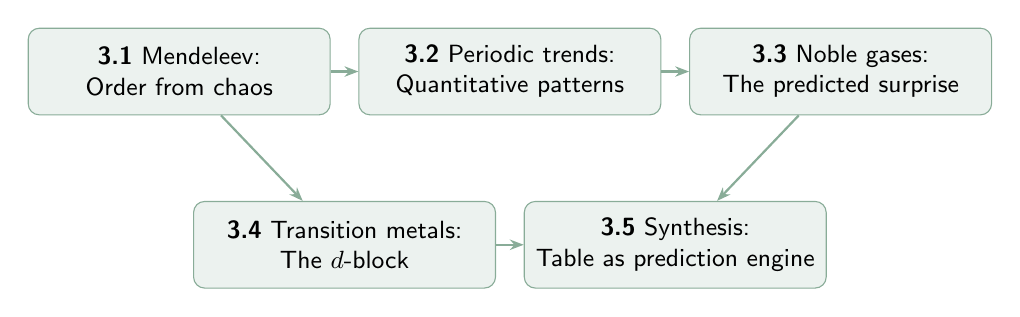
\begin{tikzpicture}[
  every node/.style={font=\sffamily\small, align=center},
  modbox/.style={draw=JourneyColor!50, fill=JourneyColor!8,
    rounded corners=4pt, minimum width=3.8cm, minimum height=1.1cm,
    text width=3.6cm},
  arr/.style={-{Stealth[length=5pt]}, thick, JourneyColor!50}
]
  \node[modbox] (m1) at (0, 0)
    {\textbf{3.1} Mendeleev:\\Order from chaos};
  \node[modbox] (m2) at (4.2, 0)
    {\textbf{3.2} Periodic trends:\\Quantitative patterns};
  \node[modbox] (m3) at (8.4, 0)
    {\textbf{3.3} Noble gases:\\The predicted surprise};
  \node[modbox] (m4) at (2.1,-2.2)
    {\textbf{3.4} Transition metals:\\The $d$-block};
  \node[modbox] (m5) at (6.3,-2.2)
    {\textbf{3.5} Synthesis:\\Table as prediction engine};

  \draw[arr] (m1) -- (m2);
  \draw[arr] (m2) -- (m3);
  \draw[arr] (m1) -- (m4);
  \draw[arr] (m3) -- (m5);
  \draw[arr] (m4) -- (m5);
\end{tikzpicture}
\end{center}

\vspace{1em}

\setcounter{section}{0}

% ══════════════════════════════════════════════════════════════════════════════
\section{Module 3.1 --- Mendeleev's Discovery: Order from Chaos}
\label{sec:mod3.1}

\subsection*{Motivation}

In 1869, sixty-three elements were known.
Their properties had been carefully measured:
atomic weights, melting points, densities, colours,
the compounds they formed, the valences they exhibited.

No two elements were the same.
The collection looked like a random assortment of facts ---
a zoo of substances with no apparent order.

Dmitri Mendeleev sat down with a set of cards,
one card per element, properties written on each.
He arranged them, rearranged them, looked for patterns.

Over a single night --- according to legend ---
he produced a table that:
\begin{itemize}[nosep, leftmargin=2em]
  \item Arranged all 63 known elements in a single coherent order.
  \item Revealed repeating patterns (periodicity) in their properties.
  \item Predicted the existence and properties of three
        elements not yet discovered.
  \item Identified errors in previously accepted atomic weights.
\end{itemize}

The periodic table is one of the greatest acts of pattern
recognition in the history of science.
This module reconstructs how Mendeleev found it.

% ─── Section: The Problem Mendeleev Faced ────────────────────────────────────
\subsection{The Problem: 63 Elements, No Framework}

By 1869, chemists had established several clusters of
similar elements:
\begin{itemize}[nosep, leftmargin=2em]
  \item \textbf{Alkali metals}: Li, Na, K --- soft, reactive,
        form similar compounds
  \item \textbf{Halogens}: F, Cl, Br, I --- reactive nonmetals,
        form salts with metals
  \item \textbf{Alkaline earths}: Be, Mg, Ca, Sr, Ba ---
        form oxides and carbonates with similar formulas
\end{itemize}

But how did these families relate to each other?
And what about the many elements that didn't fit neatly
into a family?

Earlier attempts had noticed fragments of order.
In 1864, John Newlands arranged the 56 then-known elements
by atomic weight and noticed that every 8th element
resembled the first (\newterm{Law of Octaves}).
The chemical community mocked him.
One member of the Chemical Society asked whether he had
tried arranging the elements alphabetically.

\begin{puzzlebox}
Before looking at Mendeleev's solution, try to find
the pattern yourself.

Here are the atomic weights and key properties of the
first 20 elements in order of atomic weight.
Look for repeating patterns.

\begin{center}
\small
\begin{tabular}{llccp{5cm}}
\toprule
$Z$ & Element & At.\ wt & Valence & Character \\
\midrule
1  & H  & 1.0  & 1 & reactive nonmetal, lightest gas \\
2  & He & 4.0  & 0 & inert gas \\
3  & Li & 6.9  & 1 & soft metal, reacts with water \\
4  & Be & 9.0  & 2 & hard metal, amphoteric oxide \\
5  & B  & 10.8 & 3 & metalloid, forms borates \\
6  & C  & 12.0 & 4 & nonmetal, forms vast range of compounds \\
7  & N  & 14.0 & 3 & nonmetal gas, forms \ce{NH3}, \ce{NO2} \\
8  & O  & 16.0 & 2 & reactive nonmetal, forms oxides \\
9  & F  & 19.0 & 1 & most reactive nonmetal \\
10 & Ne & 20.2 & 0 & inert gas \\
11 & Na & 23.0 & 1 & soft metal, reacts violently with water \\
12 & Mg & 24.3 & 2 & light metal, forms \ce{MgO}, \ce{MgCl2} \\
13 & Al & 27.0 & 3 & light metal, amphoteric oxide \\
14 & Si & 28.1 & 4 & metalloid, forms \ce{SiO2} \\
15 & P  & 31.0 & 3 & nonmetal, forms \ce{PH3}, \ce{P4O10} \\
16 & S  & 32.1 & 2 & nonmetal, forms \ce{H2S}, \ce{SO3} \\
17 & Cl & 35.5 & 1 & reactive nonmetal gas, forms salts \\
18 & Ar & 39.9 & 0 & inert gas \\
19 & K  & 39.1 & 1 & soft metal, more reactive than Na \\
20 & Ca & 40.1 & 2 & metal, forms \ce{CaO}, \ce{CaCO3} \\
\bottomrule
\end{tabular}
\end{center}

\begin{enumerate}[label=(\alph*), leftmargin=*]
  \item Arrange these 20 elements in a grid such that elements
        with similar valence (combining power) fall in the
        same column.
        What period lengths do you need?

  \item Identify which pairs of elements in the list
        are chemically similar.
        Is there a regular interval between them?

  \item Helium (He) and Neon (Ne) have valence 0.
        Where do they fit in your grid?
        What does this suggest about how many more
        ``valence 0'' elements might exist?

  \item Notice that $Z=19$ (K, mass 39.1) and $Z=18$ (Ar, mass 39.9):
        potassium has lower mass than argon, yet comes after it
        by chemical character.
        This was a known anomaly in 1869.
        How did Mendeleev handle anomalies like this?
\end{enumerate}
\end{puzzlebox}

% ─── Section: Mendeleev's Key Insight ────────────────────────────────────────
\subsection{Mendeleev's Key Insight: Leave Gaps}

Other chemists had tried to force all known elements
into a neat table.
Mendeleev's critical insight was to do the opposite:
when the pattern demanded it, he \emph{left gaps}
for elements that had not yet been discovered.

This required intellectual courage.
It meant asserting that the table was correct
and that nature had elements yet to be found.

\begin{namedconcept}{Mendeleev's Periodic Law (1869)}
The properties of the elements are a periodic function
of their atomic weights.

Arranging elements in order of increasing atomic weight,
similar properties recur at regular intervals.
These intervals define the \newterm{periods} of the table.
Elements in the same column (\newterm{groups}) share
characteristic chemical properties.
\end{namedconcept}

\vspace{0.5em}

Mendeleev left three prominent gaps in his 1869 table.
He named the missing elements \emph{eka-boron},
\emph{eka-aluminium}, and \emph{eka-silicon}
(``eka'' from Sanskrit, meaning ``one beyond'').

For each, he predicted:
the atomic weight, density, melting point,
oxide formula, chloride formula, and other properties ---
purely from the surrounding elements in the table.

% ─── Section: The Predictions and Their Verification ─────────────────────────
\subsection{The Predictions and Their Verification}

The most dramatic test of the periodic table was the
discovery of elements Mendeleev had predicted.

\begin{center}
\small
\begin{tabular}{lllll}
\toprule
Property & Predicted (1871) & Observed (1875) & & \\
\midrule
\multicolumn{5}{l}{\textbf{Eka-aluminium} (discovered 1875, named \textbf{Gallium})} \\
Atomic weight & 68 & 69.7 & & \\
Density (g/cm$^3$) & 5.9 & 5.91 & & \\
Melting point & low & \SI{29.8}{\degreeCelsius} (melts in hand) & & \\
Oxide formula & \ce{Ea2O3} & \ce{Ga2O3} & & \\
Solubility of oxide & dissolves in acid/base & amphoteric & & \\
\midrule
\multicolumn{5}{l}{\textbf{Eka-silicon} (discovered 1886, named \textbf{Germanium})} \\
Atomic weight & 72 & 72.6 & & \\
Density (g/cm$^3$) & 5.5 & 5.35 & & \\
Appearance & dark grey metal & grey metal & & \\
Oxide formula & \ce{EsO2} & \ce{GeO2} & & \\
Chloride formula & \ce{EsCl4}, bp $< 100$\textdegree C & \ce{GeCl4}, bp \SI{83.1}{\degreeCelsius} & & \\
\bottomrule
\end{tabular}
\end{center}

\vspace{0.5em}

When Lecoq de Boisbaudran discovered gallium in 1875,
Mendeleev pointed out that de Boisbaudran's initial
measurement of the density was wrong,
based on the predicted value.
De Boisbaudran remeasured and found Mendeleev was right.

A periodic table that could correct experimental measurements
before they were taken --- this was science operating
at its most powerful.

\begin{historybox}
\textbf{The Night of the Table}

The story that Mendeleev discovered the periodic table
in a dream is probably apocryphal, but the essential facts
are striking.

On 17 February 1869 (Russian calendar), Mendeleev was
preparing to travel to inspect cheese cooperatives
in the Russian countryside for the government
(he was a professor of chemistry who also served as
a government technical consultant).

The night before his departure, he sat down to write
a chapter of his chemistry textbook and found himself
unable to proceed without settling the arrangement of
the elements.
He spent the night arranging and rearranging his cards.
By morning he had the table.

He sent it to the Russian Chemical Society and left
to inspect the cheese cooperatives.

The table that changed chemistry was produced in one night,
as a byproduct of writing a textbook chapter,
by a man who then went to look at cheese.
\end{historybox}

% ─── Section: Reconstructing the Table ───────────────────────────────────────
\subsection{A Partial Reconstruction of the 1869 Table}

Below is a simplified version of Mendeleev's arrangement
for the first four periods.
Gaps are marked with \textbf{?} for predicted elements.

\begin{center}
\setlength{\tabcolsep}{4pt}
\small
\begin{tabular}{c|cccccccc}
\toprule
Period & Grp 1 & Grp 2 & Grp 3 & Grp 4 & Grp 5 & Grp 6 & Grp 7 & Grp 0 \\
\midrule
1 & H & & & & & & & \\
2 & Li & Be & B & C & N & O & F & \\
3 & Na & Mg & Al & Si & P & S & Cl & \\
  & & & & & & & & \\
4 & K & Ca & \cellcolor{PredictedCell}\textbf{?} & Ti & V & Cr & Mn & \\
  & & & Sc (1879) & & & & & \\
\bottomrule
\end{tabular}
\end{center}

\vspace{0.5em}

Notice the diagonal similarity:
Li--Mg, Be--Al, B--Si.
Elements diagonally adjacent in the table often share
properties because they have similar charge-to-size ratios.

% ─── Section: What Mendeleev Could Not Explain ────────────────────────────────
\subsection{What Mendeleev Could Not Explain}

The periodic law was a triumph of pattern recognition.
But Mendeleev could not explain \emph{why} the pattern existed.

\begin{itemize}[nosep, leftmargin=2em]
  \item Why do properties repeat at regular intervals?
  \item Why are the period lengths 2, 8, 8, 18, 18, 32, 32?
  \item Why do some elements (Co/Ni, Ar/K, Te/I) have
        their chemical order reversed from their mass order?
  \item Why is there a whole family of inert gases
        (not yet known in 1869) that fits between halogens
        and alkali metals?
\end{itemize}

The answer to all four questions is electron configuration
--- which was not understood until 1926.
The period lengths $2, 8, 8, 18, 18, 32, 32$ are
exactly $2n^2$ for $n = 1, 1, 2, 2, 3, 3, 4$ ---
twice the number of orbitals in each shell pair.

Mendeleev's table was right for the wrong reason.
The true reason is quantum mechanics.

\begin{discoverybox}
\textbf{Why 2, 8, 18, 32?}

From Journey 2, the number of electrons that fit in each
principal shell $n$ is $2n^2$:

\begin{center}
\begin{tabular}{ccccc}
\toprule
Shell $n$ & Subshells & Orbitals & Max electrons ($2n^2$) & Period length \\
\midrule
1 & $1s$ & 1 & 2 & 2 \\
2 & $2s$, $2p$ & 4 & 8 & 8 \\
3 & $3s$, $3p$ & 4 & 8 & 8 \\
  & ($3d$ fills later) & & & \\
4 & $4s$, $3d$, $4p$ & 9 & 18 & 18 \\
5 & $5s$, $4d$, $5p$ & 9 & 18 & 18 \\
6 & $6s$, $4f$, $5d$, $6p$ & 16 & 32 & 32 \\
\bottomrule
\end{tabular}
\end{center}

Each period corresponds to filling one set of subshells.
The period ends when a noble gas configuration is reached ---
a full set of outermost $s$ and $p$ orbitals.
\end{discoverybox}

% ─── Section: The Modern Table's Structure ────────────────────────────────────
\subsection{Reading the Modern Periodic Table}

The modern table is organised into blocks corresponding
to which subshell is being filled.

\begin{center}
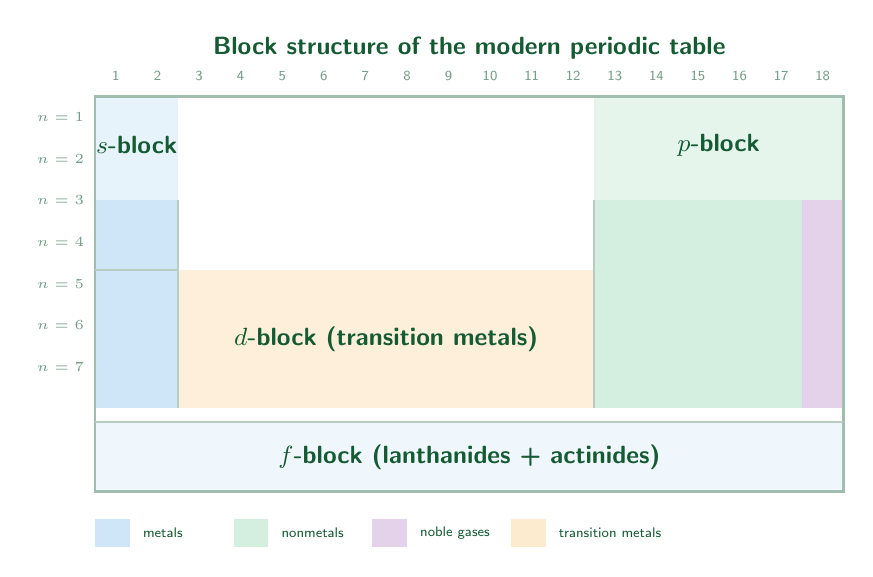
\begin{tikzpicture}[every node/.style={font=\sffamily\footnotesize},
                    scale=0.88]

  % s-block (Groups 1-2)
  \fill[TableMetal!60]  (0,0) rectangle (1.2,3.0);
  \fill[TableMetal!30]  (0,3.0) rectangle (1.2,4.5);
  \node[font=\sffamily\small\bfseries, text=JourneyColor]
    at (0.6, 3.8) {$s$-block};

  % p-block (Groups 13-18)
  \fill[TableNonmetal!50] (7.2,0) rectangle (10.8,3.0);
  \fill[TableNoble!60]    (10.2,0) rectangle (10.8,3.0);
  \fill[TableNonmetal!30] (7.2,3.0) rectangle (10.8,4.5);
  \node[font=\sffamily\small\bfseries, text=JourneyColor]
    at (9.0, 3.8) {$p$-block};

  % d-block (Groups 3-12, periods 4+)
  \fill[TableMetalloid!40] (1.2,0) rectangle (7.2,2.0);
  \node[font=\sffamily\small\bfseries, text=JourneyColor]
    at (4.2, 1.0) {$d$-block (transition metals)};

  % f-block (lanthanides/actinides, below)
  \fill[TableMetal!20] (0,-1.2) rectangle (10.8,-0.2);
  \node[font=\sffamily\small\bfseries, text=JourneyColor]
    at (5.4,-0.7) {$f$-block (lanthanides + actinides)};

  % Period labels
  \foreach \p/\y in {1/4.2, 2/3.6, 3/3.0, 4/2.4, 5/1.8, 6/1.2, 7/0.6}{
    \node[font=\sffamily\tiny, text=JourneyColor!60]
      at (-0.5,\y) {$n=\p$};
  }

  % Group labels (abbreviated)
  \foreach \g/\x in {1/0.3, 2/0.9, 13/7.5, 14/8.1, 15/8.7, 16/9.3, 17/9.9, 18/10.5}{
    \node[font=\sffamily\tiny, text=JourneyColor!60]
      at (\x, 4.8) {\g};
  }
  \foreach \g/\x in {3/1.5, 4/2.1, 5/2.7, 6/3.3, 7/3.9, 8/4.5, 9/5.1, 10/5.7, 11/6.3, 12/6.9}{
    \node[font=\sffamily\tiny, text=JourneyColor!60]
      at (\x, 4.8) {\g};
  }

  % Outer border
  \draw[thick, JourneyColor!40] (0,-1.2) rectangle (10.8,4.5);
  \draw[thick, JourneyColor!30] (0,-0.2) -- (10.8,-0.2);
  \draw[thick, JourneyColor!30] (1.2,0) -- (1.2,3.0);
  \draw[thick, JourneyColor!30] (7.2,0) -- (7.2,3.0);
  \draw[thick, JourneyColor!30] (0,2.0) -- (1.2,2.0);

  % Title
  \node[font=\sffamily\small\bfseries, color=JourneyColor]
    at (5.4, 5.2) {Block structure of the modern periodic table};

  % Legend
  \fill[TableMetal!60]     (0,-2.0) rectangle (0.5,-1.6);
  \node[right, font=\sffamily\tiny, text=JourneyColor] at (0.55,-1.8) {metals};
  \fill[TableNonmetal!50]  (2.0,-2.0) rectangle (2.5,-1.6);
  \node[right, font=\sffamily\tiny, text=JourneyColor] at (2.55,-1.8) {nonmetals};
  \fill[TableNoble!60]     (4.0,-2.0) rectangle (4.5,-1.6);
  \node[right, font=\sffamily\tiny, text=JourneyColor] at (4.55,-1.8) {noble gases};
  \fill[TableMetalloid!50] (6.0,-2.0) rectangle (6.5,-1.6);
  \node[right, font=\sffamily\tiny, text=JourneyColor] at (6.55,-1.8) {transition metals};

\end{tikzpicture}
\end{center}

\vspace{0.5em}

The key rules for reading the table:
\begin{itemize}[nosep, leftmargin=2em]
  \item \textbf{Period number} = principal quantum number of the
        outermost electrons.
  \item \textbf{Group number} (for $s$ and $p$ blocks) indicates
        how many valence electrons the element has.
  \item \textbf{Block} tells you which subshell the outermost
        electrons are in.
  \item \textbf{Position within a block} tells you how many
        electrons are in that subshell.
\end{itemize}

\begin{problembox}
\begin{enumerate}[label=\textbf{\arabic*.}]
  \item Use the periodic table's structure to determine
        the valence electron configuration of:
        \begin{enumerate}[label=(\alph*)]
          \item Phosphorus (P, $Z=15$, Period 3, Group 15)
          \item Calcium (Ca, $Z=20$, Period 4, Group 2)
          \item Iron (Fe, $Z=26$, Period 4, Group 8)
          \item Bromine (Br, $Z=35$, Period 4, Group 17)
          \item Tin (Sn, $Z=50$, Period 5, Group 14)
        \end{enumerate}

  \item The ``diagonal rule'' states that elements on the
        same diagonal of the periodic table have similar
        properties.
        \begin{enumerate}[label=(\alph*)]
          \item Lithium (Li) resembles magnesium (Mg) more
                than sodium.
                Both form only one type of stable ion
                (Li$^+$ and Mg$^{2+}$ have similar charge
                density).
                Explain in terms of their positions in the table.
          \item Beryllium (Be) resembles aluminium (Al):
                both form amphoteric oxides (dissolve in both
                acid and base), both form covalent chlorides.
                Are these elements in the same group, period,
                or neither?
        \end{enumerate}

  \item \textbf{Predicting from the table.}
        Element 114 (flerovium, Fl) is a synthetic element
        in Group 14, Period 7.
        \begin{enumerate}[label=(\alph*)]
          \item What is its predicted electron configuration?
          \item Its neighbours in Group 14 are Pb and Sn.
                Predict: Is Fl more likely to be a metal or
                nonmetal? Solid or gas at room temperature?
          \item Predict the formula of its most stable oxide
                and chloride.
          \item What is the oxidation state of the group-14
                elements in their highest oxide?
                Is this consistent down the group?
        \end{enumerate}
\end{enumerate}
\end{problembox}

% ─── Section: Where the Table Breaks Down ────────────────────────────────────
\subsection*{Where Mendeleev's Picture Breaks Down}

\begin{modelbreaks}
Mendeleev's original table ordered elements by atomic \emph{weight}.
This creates three well-known inversions:

\begin{center}
\small
\begin{tabular}{lllll}
\toprule
Pair & By mass & By $Z$ & Chemical ordering requires \\
\midrule
Ar / K  & Ar (39.9) before K (39.1) & reversed & K after Ar by chemistry \\
Co / Ni & Co (58.9) before Ni (58.7) & reversed & Ni after Co by chemistry \\
Te / I  & Te (127.6) before I (126.9) & reversed & I after Te by chemistry \\
\bottomrule
\end{tabular}
\end{center}

Mendeleev knew about these anomalies and assumed the
measured atomic weights were wrong.
They were not wrong.

The resolution came in 1913 with Moseley's X-ray experiments
(Journey~2, Module~2.7): the correct ordering criterion
is atomic number $Z$, not atomic mass.
The mass inversions arise because some heavier elements
have a higher proportion of lighter isotopes.

Mendeleev's table was correct in spirit and structure,
but used the wrong ordering parameter.
The true periodic law is: \emph{properties are periodic
functions of atomic number $Z$}.
\end{modelbreaks}

\begin{historybox}
\textbf{Henry Moseley and the atomic number.}
In 1913, 25-year-old Henry Moseley measured the wavelengths of X-rays emitted by different elements under electron bombardment. He discovered that the square root of the frequency of the $K_\alpha$ X-ray line was directly proportional to the element's position in the periodic table, an integer representing the nuclear charge $Z$. This proved that the sorting order of the elements is physically defined by nuclear proton count, not atomic weight, resolving Mendeleev's mass-reversal anomalies (like cobalt and nickel). Moseley predicted the exact positions of missing elements, but his work was cut short. He volunteered for the British army and was killed by a sniper at Gallipoli in 1915 at age 27. His death led the British government to ban prominent scientists from active combat.
\end{historybox}

% ─── Section: Deep Problems ──────────────────────────────────────────────────

\subsection*{Deep Problems}

\begin{deepbox}
\begin{enumerate}[label=\textbf{D\arabic*.}]

  \item \textbf{Mendeleev's Predictions: Quantitative Analysis.}

        Mendeleev predicted the properties of eka-silicon
        (germanium) by averaging the properties of its
        neighbours in the table.
        The neighbours of Ge in the modern table are:
        Si ($Z=14$), Sn ($Z=50$), As ($Z=33$), Ga ($Z=31$).

        Known properties:
        \begin{center}
        \small
        \begin{tabular}{lccc}
        \toprule
        Element & Atomic mass & Density (g/cm$^3$) & Melting pt (\textdegree C) \\
        \midrule
        Si & 28.1 & 2.33 & 1414 \\
        Sn & 118.7 & 7.31 & 232 \\
        As & 74.9 & 5.73 & 817 \\
        Ga & 69.7 & 5.91 & 30 \\
        \midrule
        Ge (actual) & 72.6 & 5.35 & 938 \\
        \bottomrule
        \end{tabular}
        \end{center}
        \begin{enumerate}[label=(\alph*)]
          \item Using the arithmetic mean of its four
                neighbours, predict Ge's atomic mass, density,
                and melting point.
          \item How well does this simple averaging work?
          \item Mendeleev actually used only vertical and
                horizontal neighbours (Si and Sn in Group 14;
                Ga and As in Period 4).
                Repeat the calculation using only these four.
          \item What does the success of this averaging
                tell us about the mathematical structure of
                the periodic table?
        \end{enumerate}

  \item \textbf{The Periodic Table as a Conservation Law.}

        Charge conservation, mass-energy conservation, and
        the periodic law are all ``conservation'' laws in
        a loose sense: they say that certain quantities
        are preserved or that certain structures recur.

        \begin{enumerate}[label=(\alph*)]
          \item In what sense is the periodic recurrence of
                properties a ``law'' rather than merely
                a ``pattern''?
                What distinguishes a law from a pattern?
          \item The periodic table has predictive power
                (Mendeleev predicted undiscovered elements).
                Name three other scientific frameworks that
                have predictive power of the same kind ---
                predicting unseen objects from structure alone.
          \item A physicist in 1869 who understood atomic
                structure but knew nothing of elements
                could have derived the period lengths
                $2, 8, 8, 18, \ldots$ from the Schr\"{o}dinger
                equation.
                Does this mean Mendeleev discovered an
                empirical shadow of quantum mechanics?
                What does it mean when an empirical pattern
                turns out to be a consequence of a deeper theory?
        \end{enumerate}

  \item \textbf{Island of Stability.}

        Beyond uranium ($Z=92$), all elements are synthetic
        and radioactive.
        The heaviest confirmed element is oganesson ($Z=118$).
        Nuclear physicists predict a region of increased
        stability (``island of stability'') around $Z=114$,
        $N=184$, based on nuclear shell closures.

        \begin{enumerate}[label=(\alph*)]
          \item Oganesson is in Group 18, Period 7
                (noble gas configuration $[Rn]\,5f^{14}\,6d^{10}\,7s^2\,7p^6$).
                Predict whether it behaves as a noble gas.
                (Consider: its valence electrons are in
                the $7p$ subshell, and relativistic effects
                make heavy-element electrons behave differently.)
          \item If the island of stability exists and element 126
                (unbihexium) is synthesised and found stable
                for years, where would it appear in the periodic
                table?
                What would its chemical properties be?
          \item The periodic table is currently 7 periods.
                If elements in period 8 were synthesised,
                what new block would need to be added?
                (Hint: $5g$ orbitals)
        \end{enumerate}

\end{enumerate}
\end{deepbox}

% ─── Reflection ──────────────────────────────────────────────────────────────
\subsection*{Reflection}

\begin{reflectionbox}
\begin{enumerate}[label=\textbf{R\arabic*.}]
  \item Mendeleev left gaps for elements he had never seen.
        \textbf{What gave him the right to trust the pattern
        more than the inventory of known elements?}
        Under what conditions is it rational to believe
        a pattern implies missing data, rather than to
        accept that the pattern is merely approximate?

  \item Mendeleev's table was right, but for the wrong
        reason: he ordered by mass, not by atomic number.
        The true law (properties depend on $Z$) wasn't known
        until Moseley in 1913.
        \textbf{Can a theory be correct and wrong simultaneously?}
        Is Mendeleev's periodic law the same theory as the
        modern one, or a different theory that makes the
        same predictions in most cases?

  \item The periodic table organised 63 seemingly unrelated
        substances into a coherent structure.
        \textbf{What other scientific achievements have taken
        a large collection of apparently disconnected
        observations and revealed a hidden order?}
        What do these episodes share methodologically?

  \item Mendeleev's table was rejected by some, accepted by
        others.
        It became universally accepted only after the
        predictions were confirmed.
        \textbf{What should the scientific community's
        threshold for accepting a bold, predictive claim be?}
        How much confirming evidence is enough?
\end{enumerate}
\end{reflectionbox}

\vspace{1.5em}
\begin{center}
\begin{tcolorbox}[enhanced, colback=DiscoveryColor!8, colframe=DiscoveryColor,
  width=0.88\textwidth, arc=3pt]
\centering\sffamily\small
\textbf{What we invented in this module.}\\[4pt]
We invented the idea that the elements are not a random zoo
but a structured family obeying a periodic law.
Mendeleev did not derive this from theory --- he read it
from the data, by refusing to accept chaos as the final
answer and by trusting the pattern enough to leave gaps.
The periodic table is a prediction machine.
It has predicted the existence of entire groups of elements
(noble gases, discovered 1894--1898), the ordering of known
elements (Moseley, 1913), and the properties of synthetic
elements not yet made (flerovium, 2012).
The reason it works is quantum mechanics.
But it was discovered by pattern recognition alone,
27 years before the electron was found.
\end{tcolorbox}
\end{center}

\vspace{2em}
\noindent\textcolor{JourneyColor!40}{\rule{\textwidth}{0.6pt}}
\begin{center}
\textit{\sffamily\small
Module 3.1 complete. Continue to Module 3.2:\\
\textbf{Periodic Trends: Reading the Table Quantitatively}.}
\end{center}

\end{document}